\documentclass{beamer}
\usepackage[utf8]{inputenc}
\usepackage[T2A]{fontenc}
\usepackage[russian]{babel}
\usepackage{graphicx}
\usepackage{array}
\usepackage{booktabs}
\usepackage{caption}
\usepackage{amsmath, amssymb}
\usepackage{mathtext}
\usepackage{cmap}

\definecolor{deepblue}{RGB}{50, 110, 180}
\definecolor{lightblue}{RGB}{70, 130, 200}
\definecolor{gold}{RGB}{255, 200, 50}
\definecolor{teal}{RGB}{0, 150, 180}

\usetheme{Madrid}
\usecolortheme{default}

\setbeamercolor{title}{fg=gold, bg=deepblue}
\setbeamercolor{frametitle}{fg=gold, bg=deepblue}
\setbeamercolor{structure}{fg=lightblue}
\setbeamercolor{block title}{fg=white, bg=lightblue}
\setbeamercolor{block body}{fg=deepblue, bg=lightblue!10}
\setbeamercolor{alerted text}{fg=gold}
\setbeamercolor{itemize item}{fg=teal}
\setbeamercolor{itemize subitem}{fg=teal!70}

\setbeamerfont{title}{size=\Large, series=\bfseries}
\setbeamerfont{frametitle}{size=\large, series=\bfseries}
\setbeamerfont{block title}{series=\bfseries}

\setbeamerfont{itemize/enumerate body}{size=\small}
\setbeamerfont{itemize/enumerate subbody}{size=\footnotesize}

\setbeamertemplate{itemize items}[triangle]
\setbeamertemplate{itemize subitem}[circle]
\title{История Орловского государственного университета \\ им. И.С. Тургенева}
\author{А.Д.~Шестаков}
\institute{Орловский государственный университет имени И. С. Тургенева}
\date{4 мая 2026}

\begin{document}

{
\setbeamercolor{background canvas}{bg=deepblue}
\begin{frame}
    \titlepage
\end{frame}
}

\begin{frame}{Начало высшего образования в Орле}
    \begin{columns}[T]
        \column{0.55\textwidth}
        \begin{itemize}
            \item \textbf{1916–1917 гг.} — инициатива интеллигенции о создании народного университета-политехникума.
            \item \textbf{7 сентября 1918 г.} — доклад в Губисполком о создании классического университета.
            \item \textbf{31 октября 1918 г.} — создан Орловский Пролетарский университет им. В.И. Ленина.
            \item \textbf{23 июня 1919 г.} — решение о создании Орловского государственного университета.
        \end{itemize}
        
        \begin{block}{Важно}
            \centering \small 5 ноября 1918 г. — день открытия
        \end{block}
        
        \column{0.4\textwidth}
        \begin{center}
            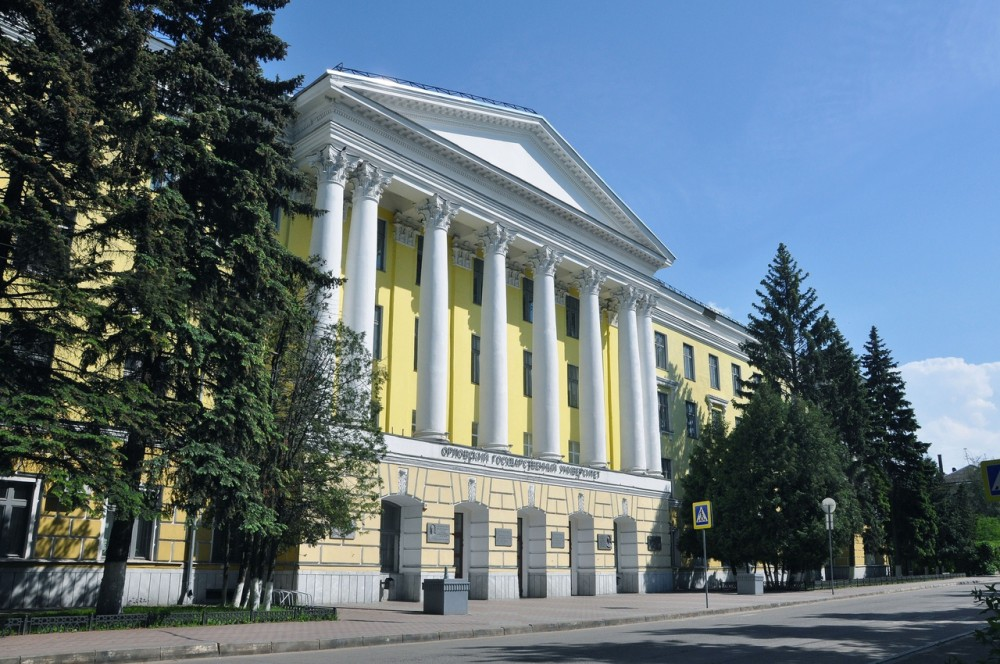
\includegraphics[height=0.35\textheight]{photo.png}
        \end{center}
    \end{columns}
\end{frame}

\begin{frame}{От университета к педагогическому институту}
    \begin{itemize}
        \item \textbf{1921 г.} — на базе ОГУ создан Высший педагогический институт.
        \item \textbf{1922 г.} — институт закрыт, студенты переведены в техникумы.
        \item \textbf{5 августа 1931 г.} — создан \textbf{Орловский индустриально-педагогический институт}.
        \item \textbf{1934 г.} — разделение на учительский и педагогический институты.
        \item \textbf{1940 г.} — первые «Учёные записки» ОГПИ.
        \item \textbf{Июнь 1941 г.} — 200 студентов и преподавателей ушли на фронт.
    \end{itemize}
    
    \begin{alertblock}{Эвакуация}
        23 августа 1941 г. — эвакуация ОГПИ в г. Бирск (Башкирская АССР)
    \end{alertblock}
\end{frame}

\begin{frame}{ОГУ в Великую Отечественную войну и после}
    \begin{columns}[T]
        \column{0.55\textwidth}
        \begin{itemize}
            \item \textbf{20 ноября 1943 г.} — реэвакуация в Елец.
            \item \textbf{Август 1944 г.} — возвращение в Орёл.
            \item \textbf{1945 г.} — первый послевоенный сборник «Учёных записок».
            \item \textbf{1945 г.} — первая докторская диссертация.
            \item \textbf{1952 г.} — переименование в \textbf{Орловский государственный педагогический институт}.
        \end{itemize}
        
        \begin{exampleblock}{Достижение}
            \centering \small Первая докторская диссертация — 1945 г.
        \end{exampleblock}
        
        \column{0.4\textwidth}
        \begin{center}
            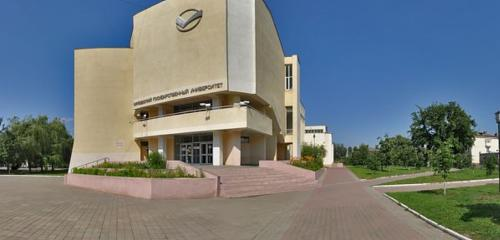
\includegraphics[width=\textwidth]{photo2.png}
            {\tiny Современное здание университета}
        \end{center}
    \end{columns}
\end{frame}

\begin{frame}{Ключевые годы истории ОГУ}
    \begin{table}
    \centering
    \begin{tabular}{p{1.2cm}|p{8cm}}
        \toprule
        \textbf{Год} & \textbf{Событие} \\
        \midrule
        1919 & Основание Орловского государственного университета \\
        1931 & Создание Орловского индустриально-педагогического института \\
        1981 & Награждение ОГПИ орденом «Знак Почёта» \\
        1994 & Получение статуса педагогического университета (ОГПУ) \\
        1996 & Преобразование в классический университет \\
        2016 & Создание Опорного университета – \textbf{ОГУ имени И.С. Тургенева} \\
        \bottomrule
    \end{tabular}
    \caption{Основные исторические преобразования вуза}
    \end{table}
\end{frame}

\begin{frame}{ОГУ им. И.С. Тургенева сегодня}
    \begin{columns}[T]
        \column{0.55\textwidth}
        \begin{itemize}
            \item \textbf{2010–2015 гг.} — реорганизация: ОрёлГТУ $\rightarrow$ Университет УНПК $\rightarrow$ Приокский государственный университет.
            \item \textbf{1 апреля 2016 г.} — создание \textbf{Опорного университета}.
        \end{itemize}
        
        \begin{block}{Награды университета}
            \begin{itemize}
                \item Орден «Знак Почёта» (1981)
                \item Премия Правительства РФ (2002)
                \item Премия Президента РФ (2003)
            \end{itemize}
        \end{block}
        
        Сегодня — ведущий вуз Орловской области.
        
        \column{0.4\textwidth}
        \begin{center}
            
\includegraphics[width=0.8\textwidth]{logo.png}\\
            \vspace{0.3cm}
            {\tiny Логотип университета}
        \end{center}
    \end{columns}
\end{frame}

\end{document}
